\documentclass{article}
\usepackage[T1]{fontenc}
\usepackage{lmodern}
\usepackage{graphicx}
\usepackage{amsmath,amssymb}
\usepackage[a4paper,margin=2cm]{geometry}
\usepackage[absolute,overlay]{textpos}
\setlength{\TPHorizModule}{1mm}
\setlength{\TPVertModule}{1mm}
\usepackage[indonesian]{babel}
\usepackage{hyperref}
\setlength{\emergencystretch}{2em}
% unit: Halaman 91

\begin{document}

% === Halaman 91 (python/native) ===

Perbedaan  ChaCha dengan Salsa:

 1. Initial state

2. Quarter round QR

91

a  a + b;   d  d  a;   d  d <<< 16;

c  c + d;    b  b  c;   b  b <<< 12;

a  a + b;    d  d  a;  d  d <<< 8;

c  c + d;     b b  c;   b  b <<< 7;

% deskripsi: gambar native xref 348
\noindent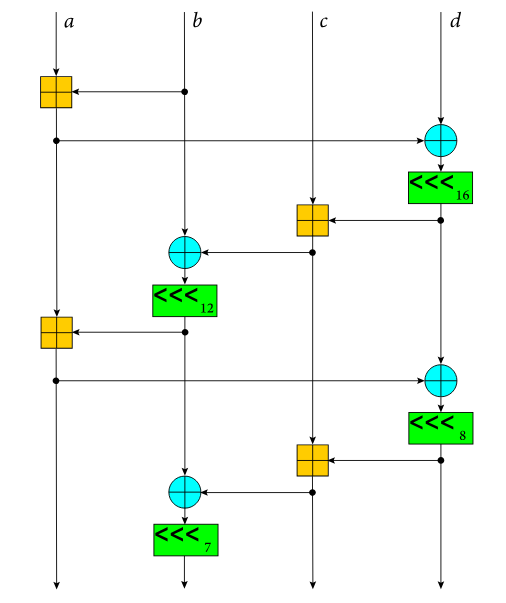
\includegraphics[width=0.85\textwidth]{../../images/python/page_091_img_01.png}

% deskripsi: gambar native xref 349
\noindent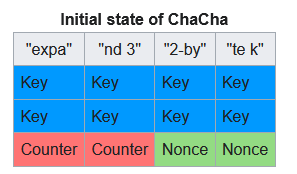
\includegraphics[width=0.85\textwidth]{../../images/python/page_091_img_02.png}

\end{document}
